\documentclass[12pt,a4paper,final]{report}			%definire grandezza testo, foglio e tipo di testo.
\usepackage[left=2.6cm,right=2.6cm]{geometry}
\usepackage{pdf14}
\usepackage[utf8]{inputenc}			%definisce la codifica dei caratteri
\usepackage[italian]{babel}				%definisce il pacchetto della lingua
\usepackage{amsmath}						%contiene molti utili strumenti per la scrittura matematica
\usepackage{amsfonts}
\usepackage{amssymb}
\usepackage{makeidx}
\usepackage{units} 					%unita di misura
\usepackage{subcaption}  		%per le figure
\usepackage{subcaption}		%DON'T KNOW. INVESTIGATE
\usepackage{siunitx} 				%unita SI
\usepackage{mathrsfs}			%per usare cose tipo \mathscr{}
\usepackage{physics}				%contiene molta notazione utile; lo uso in particolare per \bra e \ket
\usepackage{cite}
\usepackage{comment}
\usepackage{caption}
\usepackage[font=small,labelfont=bf]{caption}		% serve per ridurre la dimensione delle captions
\usepackage[final]{pdfpages}		%per poter includere pdf
\usepackage[a-1a]{pdfx}
\usepackage[pdfa]{hyperref}
%\pdfminorversion=4

\title{Riassunto di tesi}

\begin{document}
\begin{center}
	\LARGE \textbf{Stima delle proprietà di sistemi ottici nelle microonde tramite l'utilizzo di reti neurali}
	%\textbf{Stima delle proprietà di sistemi ottici nelle microonde tramite l'utilizzo di reti neurali.}
\end{center}
\begin{center}
	\normalsize \textit{Eleonora Gatti}
\end{center}

\vspace{5mm}

%CMB
La \textbf{CMB}, Cosmic Microwave Background, \`e la radiazione a microonde di fondo cosmico che permea l’intero Universo, originatasi dal disaccoppiamento tra materia e radiazione, avvenuto circa 380\,000 anni dopo il Big Bang. Lo studio della CMB è estremamente importante perché consente di studiare le condizioni in cui l'Universo si è formato, andando a caratterizzare i suoi parametri fisici in tempi molto prossimi al Big Bang (fino a $10^{-30}\,\text{s}$).


%DIAGRAMMA RADIAZIONE

\begin{comment}
Mettiti nella prospettiva di un lettore che non sa nulla di queste cose (ad esempio, un membro di commissione che fa fisica dell'atmosfera, o fisica dello stato solido): stai dando per scontati troppi concetti. Prova a metterlo così:«Negli esperimenti di CMB, e più in generale in qualsiasi esperimento di radioastronomia, è molto importante non solo misurare il segnale, ma anche ricostruire accuratamente la sua direzione di provenienza. La risposta ottica di un sistema si quantifica solitamente tramite il cosiddetto fascio d'antenna, una funzione matematica $\gamma$che associa a una direzione sulla sfera celeste $(\theta, \phi)$ un numero puro che indica l'efficienza nel catturare la radiazione: $\gamma(\theta, \phi) = 1$ se l'efficienza è massima, $\gamma(theta, \phi) = 0$ se lo strumento è cieco lungo tale direzione.»
\end{comment}

Negli esperimenti di CMB, e più in generale in qualsiasi esperimento di radioastronomia, è molto importante non solo misurare il segnale, ma anche ricostruire accuratamente la sua direzione di provenienza. La risposta ottica di un sistema si quantifica solitamente tramite il cosiddetto fascio d'antenna, una funzione matematica $\gamma$ che associa a una direzione sulla sfera celeste $(\theta, \phi)$ un numero puro che indica l'efficienza nel catturare la radiazione: $\gamma(\theta, \phi) = 1$ se l'efficienza è massima, $\gamma(\theta, \phi) = 0$ se lo strumento è cieco lungo tale direzione. La funzione $\gamma(\theta, \phi)$ definisce il \textbf{diagramma di radiazione}. Tale diagramma mostra tipicamente la presenza di un \textit{main beam}, un lobo principale nella posizione del polo nord ($\theta = 0$), nel quale è contenuta la maggior parte della radiazione.

%PARAMETRI

\begin{comment}
Rivedi questo testo alla luce della nota precedente: (1) parli di «main beam» senza averlo definito, (2) parli di "x" e "y" senza aver detto cosa sono (e probabilmente non è necessario, basta dire che l'ellitticità misura il livello di simmetria intorno all'asse del main beam). Parli di "software per la simulazione di sistemi ottici" senza che sia chiaro a cosa servono («simulano la propagazione della radiazione in un sistema ottico, consentendo di stimare $\gamma(\theta, \phi)$»), (3) dici che bisogna simulare migliaia di detector senza dire perché ne servano così tanti.
\end{comment}

A partire dal diagramma di radiazione si definiscono alcuni parametri che permettono una sua descrizione. I parametri analizzati in questo lavoro di tesi sono: la \textbf{Full Width Half Maximum} (FWHM) del main beam che è la larghezza angolare a metà della sua altezza; l'\textbf{ellitticità}, che misura il livello di simmetria intorno all'asse del main beam; la componente \textbf{co-polare massima}; la componente \textbf{cross-polare massima}.


%SIMULAZIONI

I software per la simulazione di sistemi ottici simulano la propagazione della radiazione in un sistema ottico, consentendo di stimare $\gamma(\theta, \phi)$. 
Tuttavia sono molto dispendiosi in termini di tempo e per sistemi ottici complessi, con migliaia di detector sulla superficie focale, risulta impossibile una simulazione completa dell'ottica.
Allo stesso tempo per raggiungere sensibilità strumentali elevate che consentano di rivelare segnali molto deboli, come ad esempio la stessa CMB, è fondamentale avere a disposizione vasti piani focali che permettano di utilizzare un elevato numero di rivelatori.

\`E quindi forte la necessità di trovare una via alternativa che consenta di stimare i parametri che descrivono il beam in una qualsiasi posizione.

%OBIETTIVO
L'obiettivo di questa tesi è quello di stabilire un criterio per discriminare la bontà dei diversi metodi di stima dei parametri del diagramma di radiazione, e di individuare metodi più rapidi per la stima di $\gamma(\theta, \phi)$, o almeno dei suoi parametri più rappresentativi. In particolare ho voluto verificare se una rete neurale riuscisse a predire i parametri di interesse più efficacemente rispetto ad un'interpolazione.

%DATASET
Ho effettuato le analisi a partie da un dataset, prodotto tramite il software GRASP, nel quale sono riportati i dati relativi all'ottica di STRIP, uno strumento ideato per effettuare misure di CMB a grandi scale angolari.
Nel suddetto dataset sono presenti i parametri del beam elencati sopra (FWHM, ellitticità, \ldots) in diversi punti della superficie focale, espressi come coordinate $(x,y,z)$ in uno spazio cartesiano e sono distributi su una griglia $13\text{x}13$ lungo le componenti $x$ e $y$. La griglia ha una dimensione di $\sim 70 \unit{cm}\text{x}70 \unit{cm}$, mentre la coordinata $z$ varia tra $0$ e $50 \unit{mm}$.
Attraverso tale dataset ho creato due subsets per effettuare rispettivamete l'interpolazione/training della rete e la verifica della bontà dei dati stimati.

%PROCEDURA
Per stimare le proprietà di un diagramma di radiazione attraverso strumenti classici di interpolazione ho utilizzato due metodi: \texttt{interp2d} del modulo \texttt{scipy.interpolate}, basato su un'interpolazione lineare tra punti adiacenti, e \texttt{curve\_fit} del modulo \texttt{scipy.optimize}, con cui ho fatto un fit ai minimi quadrati tra i dati e un paraboloide. Dal momento che \texttt{interp2d} ha mostrato problemi, soprattutto per i punti ai bordi del piano focale, nel resto della mia analisi ho trascurato di includerlo nei confronti.


Parallelamente ho stimato il valore dei parametri attraverso reti neurali di tipo \textit{feed forward} e \textit{fully connected}.
Ho creato 6 diverse architetture di rete che variano per funzione di attivazione (\textit{Tanh} o \textit{Sigmoid}) e numero di hidden layers (1, 2, 3). 
I risultati che ho ottenuto mostrano che le reti neurali hanno prestazioni migliori rispetto ai metodi di interpolazione, o al più equiparabili.
Il grafico sotto riportato mostra la distribuzione degli errori relativa ad uno dei parametri elencati sopra (ellitticità), confrontata tra diversi tipi di reti neurali (in blu) e il caso migliore dell'interpolazione (in arancione).

\begin{comment}
Quanto hai scritto qui va bene, ma in un riassunto di tesi questo livello di dettaglio è solitamente più del richiesto. Dì semplicemente che i tuoi risultati mostrano che le reti neurali hanno prestazioni migliori rispetto ai metodi di interpolazione, e dì che il grafico sotto mostra la distribuzione degli errori relativa ad uno dei parametri elencati sopra (ellitticità), confrontata tra diversi tipi di reti neurali e il caso migliore dell'interpolazione.

Ho suddiviso dataset iniziale il \texttt{training\_set} (75\%) e \texttt{validation\_set} (25\%). Ho inoltre normalizzato i dati di output (ovveo i valori dei parametri del beam) per facilitare la convergenza della rete. Ho effettuato il training della rete su 30000 epoche rimescolando i dati del \texttt{training\_set}  e del \texttt{validation\_set} ogni 5000 epoche. 
Ho poi riassunto risultati ottenuti attraverso dei \textit{violin plots} i quali permettono di visualizzare la densità di probabilità di ottenere un determinato valore dell’errore e di confrontare, in un unico grafico, i risultati relativi all'interpolazione e quelli relativi alle varie architetture di rete. Tanto più è piccata la curva per valori bassi dell’errore, quanto più il risultato è buono.
\`E qui riportato il violin plot relativo all'ellitticità per la quale si può osservare che alcune architetture di rete (per esempio Tanh\_2L) forniscono risultati apprezzabilmente migliori rispetto a quelli ottenuti con l’interpolazione.

Confronto dell'errore tra dato stimato e dato esatto relativo all'ellitticità. Il grafico mostra il confronto tra i risultati ottenuti tramite i diversi tipi di rete neurale e tramite interpolazione.
\end{comment}

\vspace{1cm}
\begin{figure}[!ht]
    \centering
    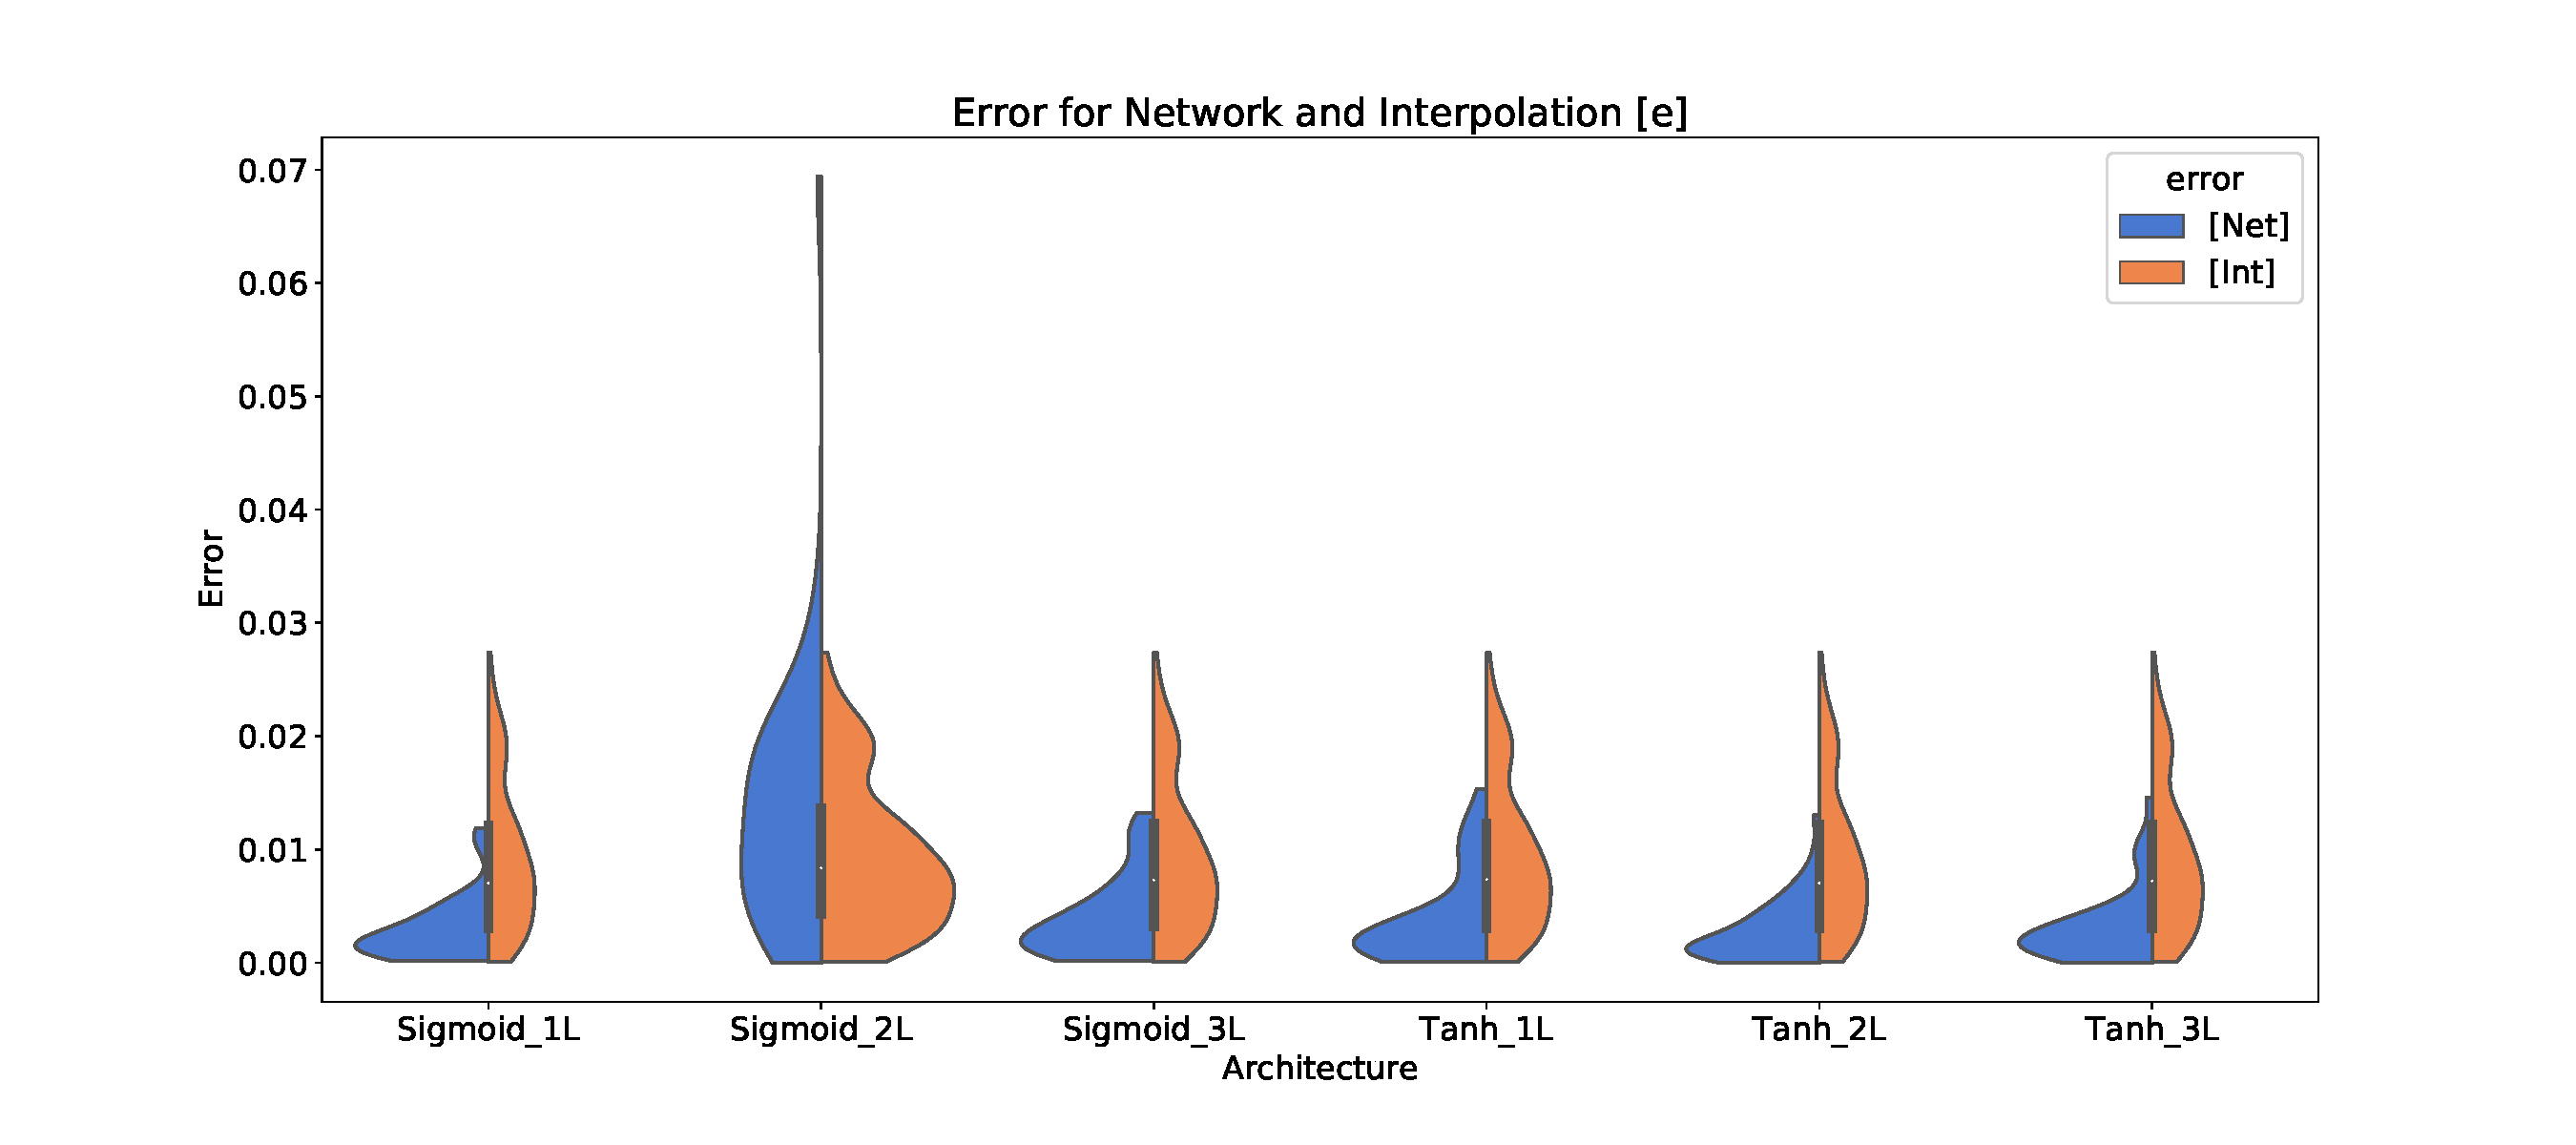
\includegraphics[width=\linewidth]{../figures/violin_plot_e.pdf}
\end{figure}


\end{document}
